\documentclass{article}

\usepackage[a4paper,margin=2cm]{geometry}
\usepackage{color, soul}
\usepackage{titlesec}
\usepackage{enumitem}
\usepackage{pdfpages}

\setitemize{itemsep=0mm}

\titlespacing*{\section}
{0pt}{2mm}{1mm}
\titlespacing*{\subsection}
{0pt}{1mm}{1mm}

\title{\vspace{-1.5cm}SWEN30006 Assignment 1 - Report}
\date{}
\author{Workshop 09, Team 02\\Lucas Fern \& Cameron Maddern}

\begin{document}
\maketitle
\noindent Implementing the required changes to the Automail system did not require the creation of any new classes in any of the existing \verb|automail|, \verb|exceptions|, or \verb|simulation| packages. Various attributes and methods were, however, added to the existing classes, and existing classes were modified. These additions will be detailed below, broken down by class. They are also highlighted in \hl{yellow} on the Design Class Diagram attached at the end of the report.

\section{Simulation}
The \verb|WifiModem| was moved out of the simulation class and into the Robot. This requires the Simulation class to import the Robot, but this slight increase in Coupling is easily justified by the significant increase in Cohesion. This is mentioned again in Section \ref{sec: robot attrs}. 
\subsection{Attributes}
The following attributes were added to the Simulation class:
\begin{itemize}
    \item \verb|private static double billableActivity|\\
         +\verb| private double activityUnitsToDeliver|\\
         +\verb| private static double activityCost|\\[2mm]
    Each of these is a statistic required to be printed at the end of the simulation. Because they aren't used elsewhere it was Cohesive to place them in the Simulation class.
\end{itemize}

\section{Automail}
The Automail constructor was modified to set an initial service fee for each floor. This incurs an upfront cost that cannot be passed on to the consumers, but is justified, as once an initial fee is set for each floor we can guarantee only one extra call will be used per delivery since a default value now exists.

\section{Robot}
The \verb|operate()| method of the Robot class was modified so that the Robot would attempt to update the service fee of the floor whenever it was completing a delivery. The \verb|moveTowards()| method was also updated so that it added the cost of each movement to the relevant variables of its MailItems.
\subsection{Attributes}
\label{sec: robot attrs}
The following attributes were added to the Robot class:
\begin{itemize}
    \item \verb|public static final double UNITS_PER_FLOOR = 5;|\\
         +\verb| public static final double UNITS_PER_LOOKUP = 0.1;|\\[2mm]
    These constants are required to update the amount of activity units for the delivery of each MailItem. They were placed here in line with the Information Expert principle, since the robot uses these after taking the relevant action to update the attributes of the items it is carrying.
    \item \verb|public static WifiModem wModem|\\[2mm]
    In this implementation of Automail the Robots are the only classes which interact with the Wi-Fi Modem except for powering it on and off. The Modem was moved into the Robot class to make them the Information Experts and increase Cohesion.
    \item \verb|private static double[] serviceFees|\\[2mm]
    This array stores the service fees most recently retrieved by a robot for each floor. This needs to be accessed by all robots, and isn't specific to each one. It was made \verb|static| to the Robot class to adhere to the High Cohesion and Information Expert patterns.
\end{itemize}
\subsection{Methods}
The following method was also added to the Robot class:
\begin{itemize}
    \item \verb|public static int attemptSetServiceFee(int floor)|\\[2mm]
    This method interacts with other \verb|static| attributes and methods of the Robot class. It was highly cohesive to place this method here.
\end{itemize}

\section{MailItem}
The existing \verb|toString()| method of the MailItem was overloaded to take an argument specifying whether to print the charge statistics. The default \verb|toString()| method was overridden to call the overloaded method with backwards compatible behaviour. This was an example of protected variation as the old interface was maintained.
\subsection{Attributes}
The following attributes were added to the MailItem class:
\begin{itemize}
    \item \verb|private double serviceFee|\\
         +\verb| private double activityUnitsToDeliver|\\[2mm]
    Each MailItem stores, updates, and operates on its own service fee and required activity units, so these were placed to obey the Information Expert principle and maintain High Cohesion.
    \item \verb|public static final double ACTIVITY_PRICE = 0.224;|\\
    +\verb| public static final double MARKUP_PROP = 0.059;|\\[2mm]
    These attributes are used in the calculation of charges upon successful deliveries, as well as in charge estimation for determining priority items. These calculations are performed by the MailItem, so it was highly cohesive to store the constants here. It was also mentioned that the system should be designed so that the weight of the items could be factored into the charge in the future. Since the weight is stored here also, this decision takes into account the cohesion of future updates.
\end{itemize}
\subsection{Methods}
The following method was also added to the MailItem class:
\begin{itemize}
    \item \verb|public static int attemptSetServiceFee(int floor)|\\[2mm]
    This method interacts with other \verb|static| attributes and methods of the MailItem class. It was highly cohesive to place this method here.
    \item \verb|public void increaseActivityUnitsToDeliver(double increase)|\\
    +\verb| private double calculateTotalActivityUnits()|\\
    +\verb| private double estimateActivityToDeliver()|\\
    +\verb| public double calculateActivityCost(double activityUnits)|\\
    +\verb| private double calculateCost(double activityUnits)|\\
    +\verb| public double calculateCharge(double activityUnits)|\\[2mm]
    These methods all operate on and make calculations based on an individual MailItem and its properties such as destination and the activity units required to move it there. These methods must take acitivtyUnits as there are multiple ways of calculating this value (estimate and actual value) It was in line with the Information Expert principle to place these methods in the same class.
\end{itemize}

\section{MailPool}
The \verb|loadItem()| method of the MailPool was modified to support priority dispatch of MailItems with a charge above the threshold defined in the configuration file. By keeping the same interface into the \verb|loadItem()| method, this variation was protected from causing adverse effects elsewhere in the Automail system.
\subsection{Methods}
The following method was also added to the MailPool class:
\begin{itemize}
    \item \verb|private boolean isPriority(MailItem item)|\\[2mm]
    This method compares the charge on a mail item to the threshold value for priority mail. It was highly cohesive to place this method here.
\end{itemize}

\section{Additional Choices}
\begin{itemize}
    \item It was decided that customers would be charged an amount proportional to the amount of floors that the robot travelled with their item, and if the robot was carrying multiple items both customers would be charged for each movement. This is because in a real life environment customers would feel ripped-off if they usually received a 50\% discount from the robot delivering two items at once, and then occasionally were charged the full price when the robot was forced to make a trip with only one item. On top of that, providing no discount is profitable for Delivering Solutions Inc.
\end{itemize}

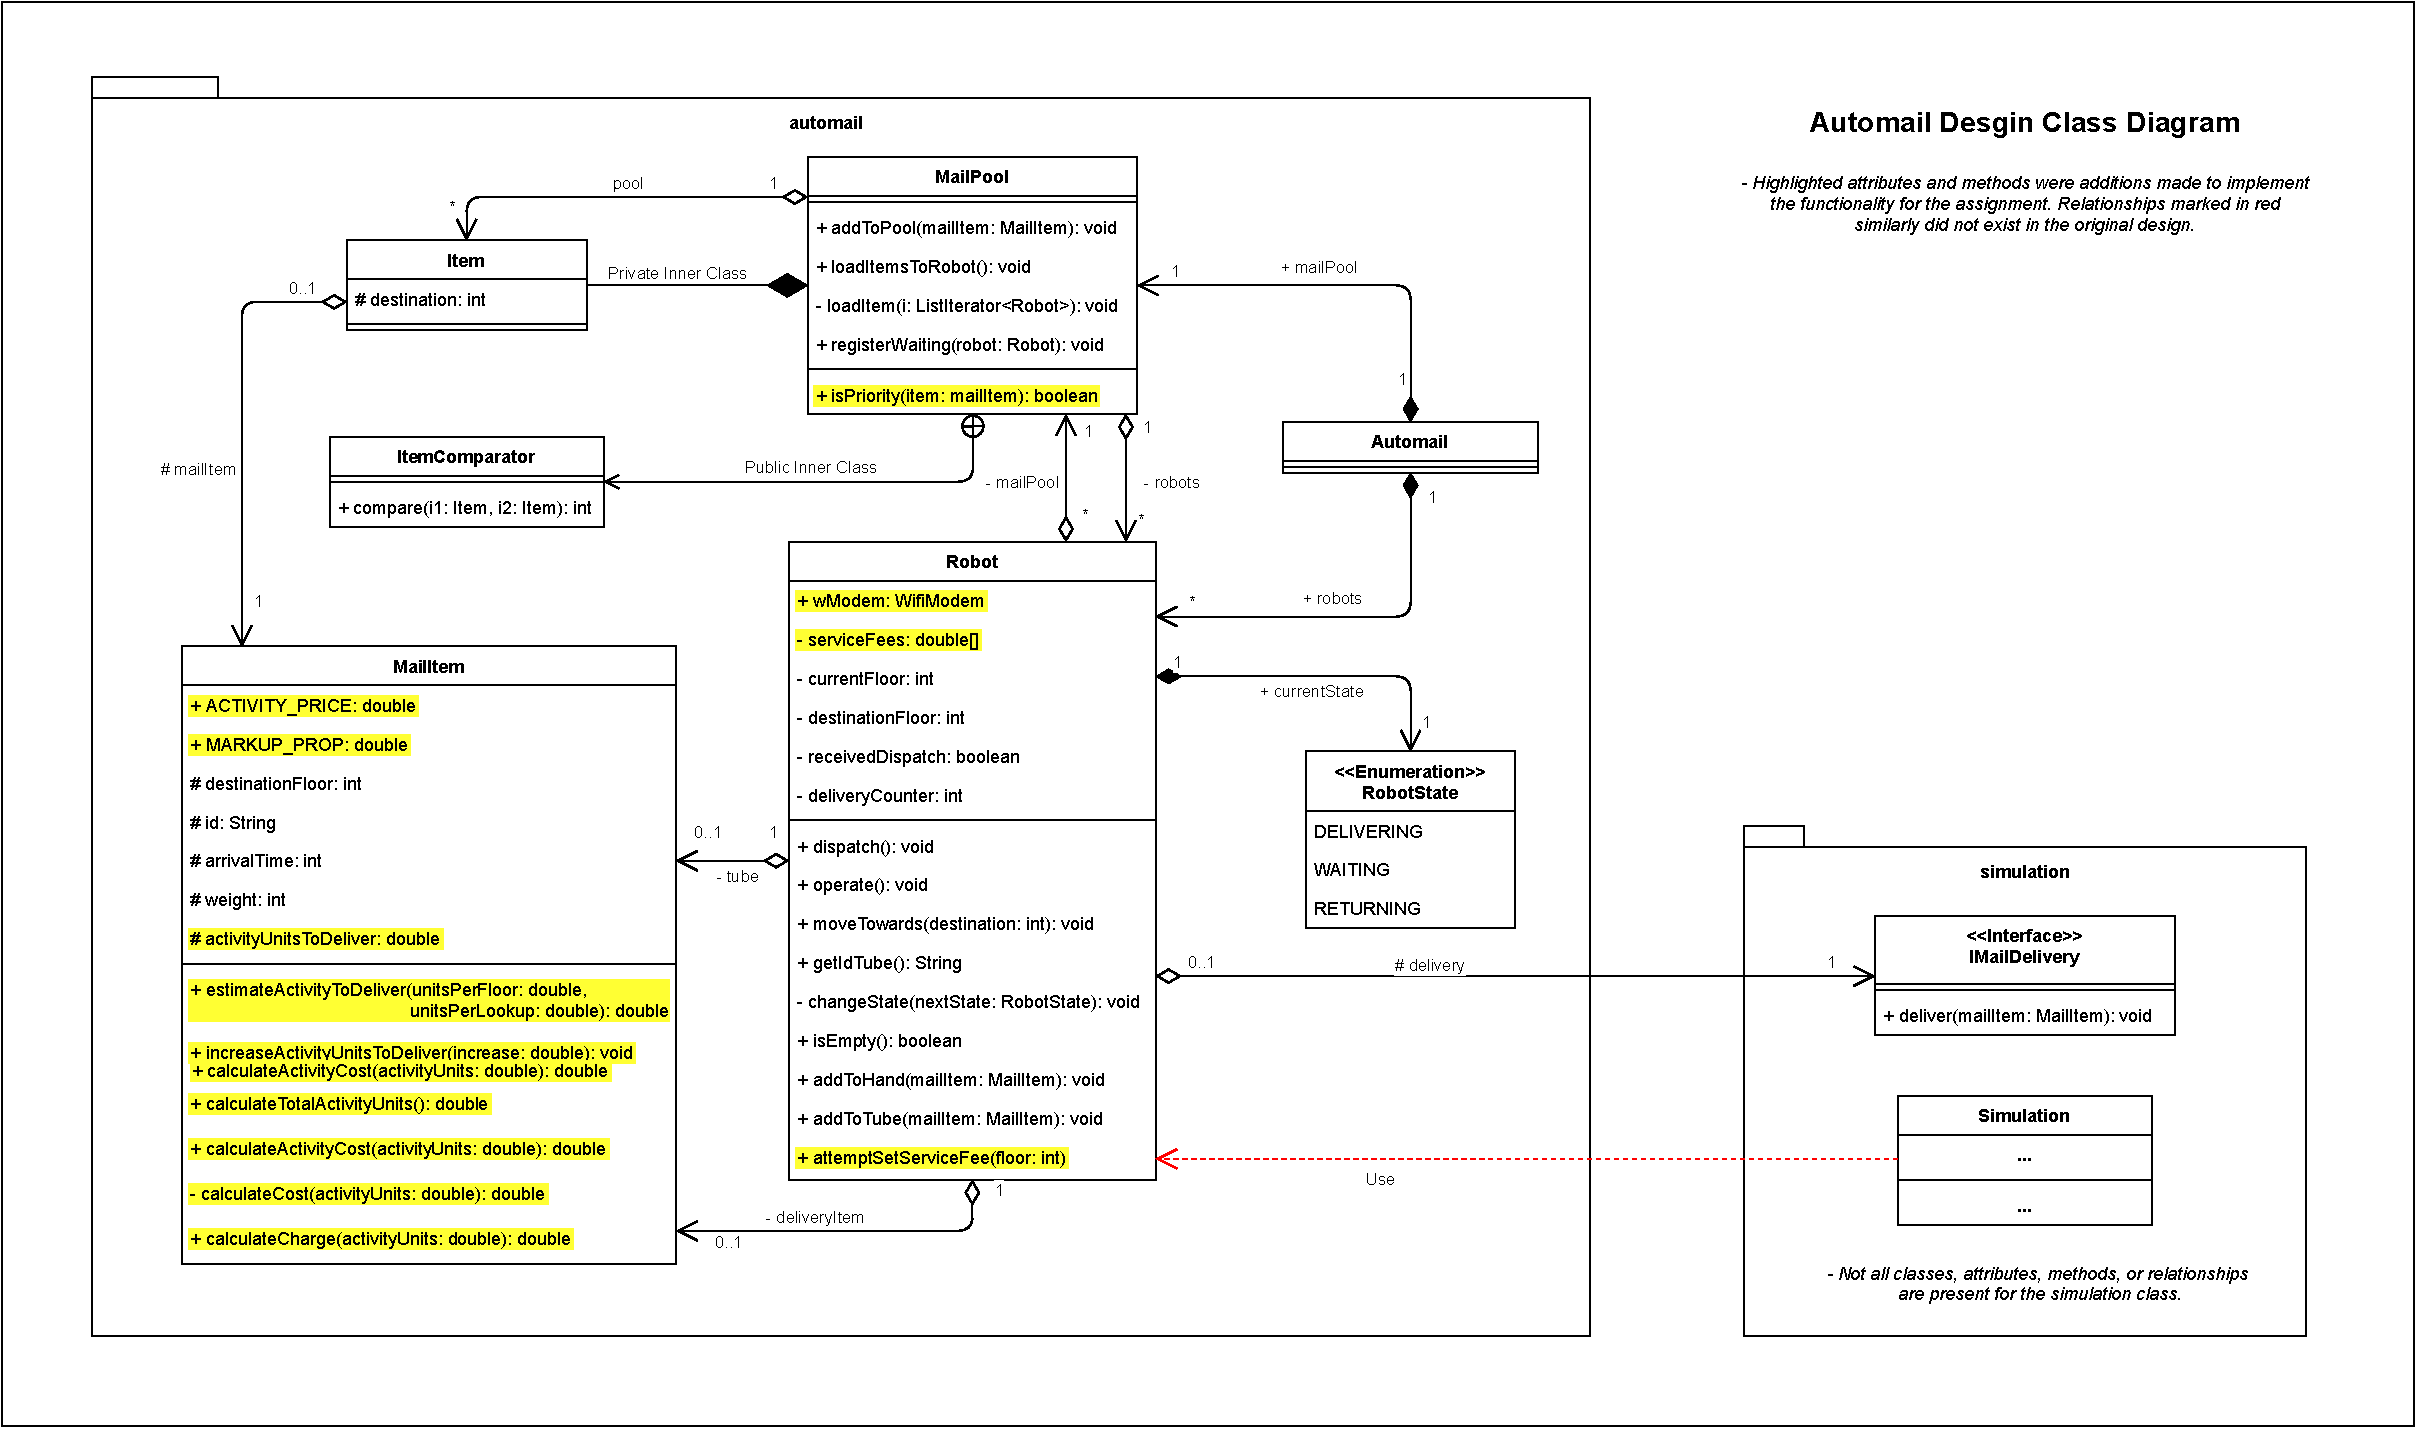
\includepdf[pages=-, fitpaper=true]{design-class-diag.pdf}
\end{document}